\documentclass{article}
% translate with >> pdflatex -shell-escape <file>

% This file is an extract of the PGFPLOTS manual, copyright by Christian Feuersaenger.
% 
% Feel free to use it as long as you cite the pgfplots manual properly.
%
% See
%   http://pgfplots.sourceforge.net/pgfplots.pdf
% for the complete manual.
%
% Any required input files (for <plot table> or <plot file> or the table package) can be downloaded
% at
% http://www.ctan.org/tex-archive/graphics/pgf/contrib/pgfplots/doc/latex/
% and
% http://www.ctan.org/tex-archive/graphics/pgf/contrib/pgfplots/doc/latex/plotdata/

\usepackage{pgfplots}
\pgfplotsset{compat=newest}

\pagestyle{empty}

\begin{document}
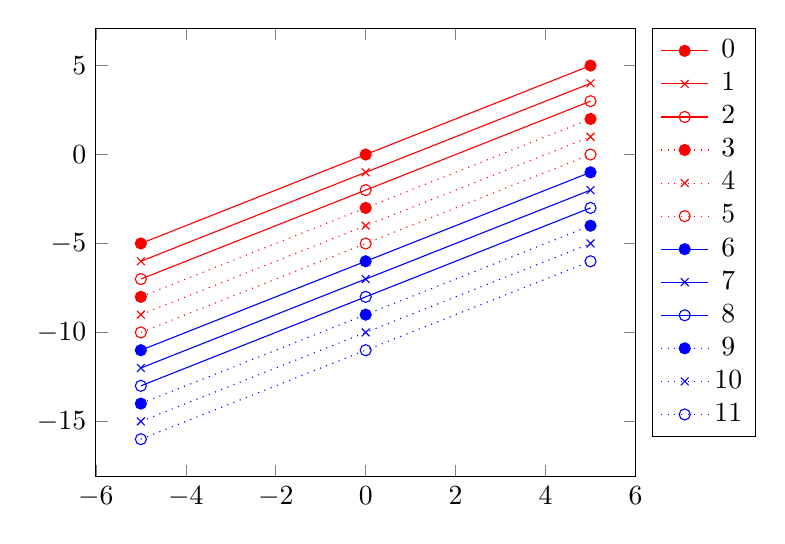
\begin{tikzpicture}
\begin{axis}[
	cycle multi list={
	  red,blue\nextlist
	  solid,{dotted,mark options={solid}}\nextlist
	  mark=*,mark=x,mark=o
	},
	samples=3,
	legend entries={0,...,20},
	legend pos=outer north east
]
	\addplot {x};
	\addplot {x-1};
	\addplot {x-2};
	\addplot {x-3};
	\addplot {x-4};
	\addplot {x-5};
	\addplot {x-6};
	\addplot {x-7};
	\addplot {x-8};
	\addplot {x-9};
	\addplot {x-10};
	\addplot {x-11};
\end{axis}
\end{tikzpicture}
\end{document}
